% Marco Teorico.
\chapter{Marco te'orico} \label{chap:ssimilar}

\vspace{5 mm}

\section{Data Clustering} \label{sect:dclust}

\subsection{Introducci\'on} \label{sect:dclusti}

Data clustering (o s\'olo clustering), tambien llamado an\'alisis de clusters, an\'alisis de segmentaci\'on,
an\'alisis de taxionom\'ia, o clasificaci\'on no supervisada, es un m\'etodo de crear grupos de objetos,
o clusters, de tal manera que cada los objetos dentro de un cluster sean similares y los objetos 
en clusters distintos sean diferents. \cite{GaChJi2007}

En \cite{SwAjAm2009} hablan de ciertos puntos importantes:

\begin{itemize}

\item Hay muchas definciones porpuestas por una diversa cantidad de personas,
 lo que demuestra la dificultad de proveer una \'unica definici\'on formal. Ésto radica en que
es bastante complejo capturar por los medios de cualquier criterio individual que se 
use la noci\'on que tiene un humano. El siguiente ejemplo va a poner en claro.

Considere los siguientes animales: oveja, perro, gato (mam\'iferos), gorri\'on, gaviota (aves),
v\'ivora, lagarto (rept\'iles), pez de colores, salmonete, tibur\'on azul (peces), y rana (anf\'ibio).
Para organizar estos animales en clusters, se tiene que definir un criterio. Por ello, si 
empleamos la manera en que estos animales llevan a cabo su descendencia, la oveja, perro, gato
y tibur\'on azul van a ser asignados al mismo cluster, mientras que el resto van a dormar un segundo
(Figura \ref{fig:ejemplo1}).  En cambio, si el criterio es la existencia de pulmones, 
el pez de colores, el salmonete y el tibur\'on son
asignados al mismo cluster, mientras que el resto a otro (Figura \ref{fig:ejemplo2}).
 Por otro lado, si el criterio es el ambiente
donde viven los anoamles, la oveja, perro, gato, gorri\'on, gaviota, v\'ivora y el lagarto van a formar un cluster
(viven fuera del agua), el pez de colores, salmonete y el tibur\'on azul van a formar un otro (viven afuera
del agua), y un tercero que va a contener a la rana, ya que puede vivir en los dos (Figura \ref{fig:ejemplo3}). 

\begin{figure}[htb]
\centering
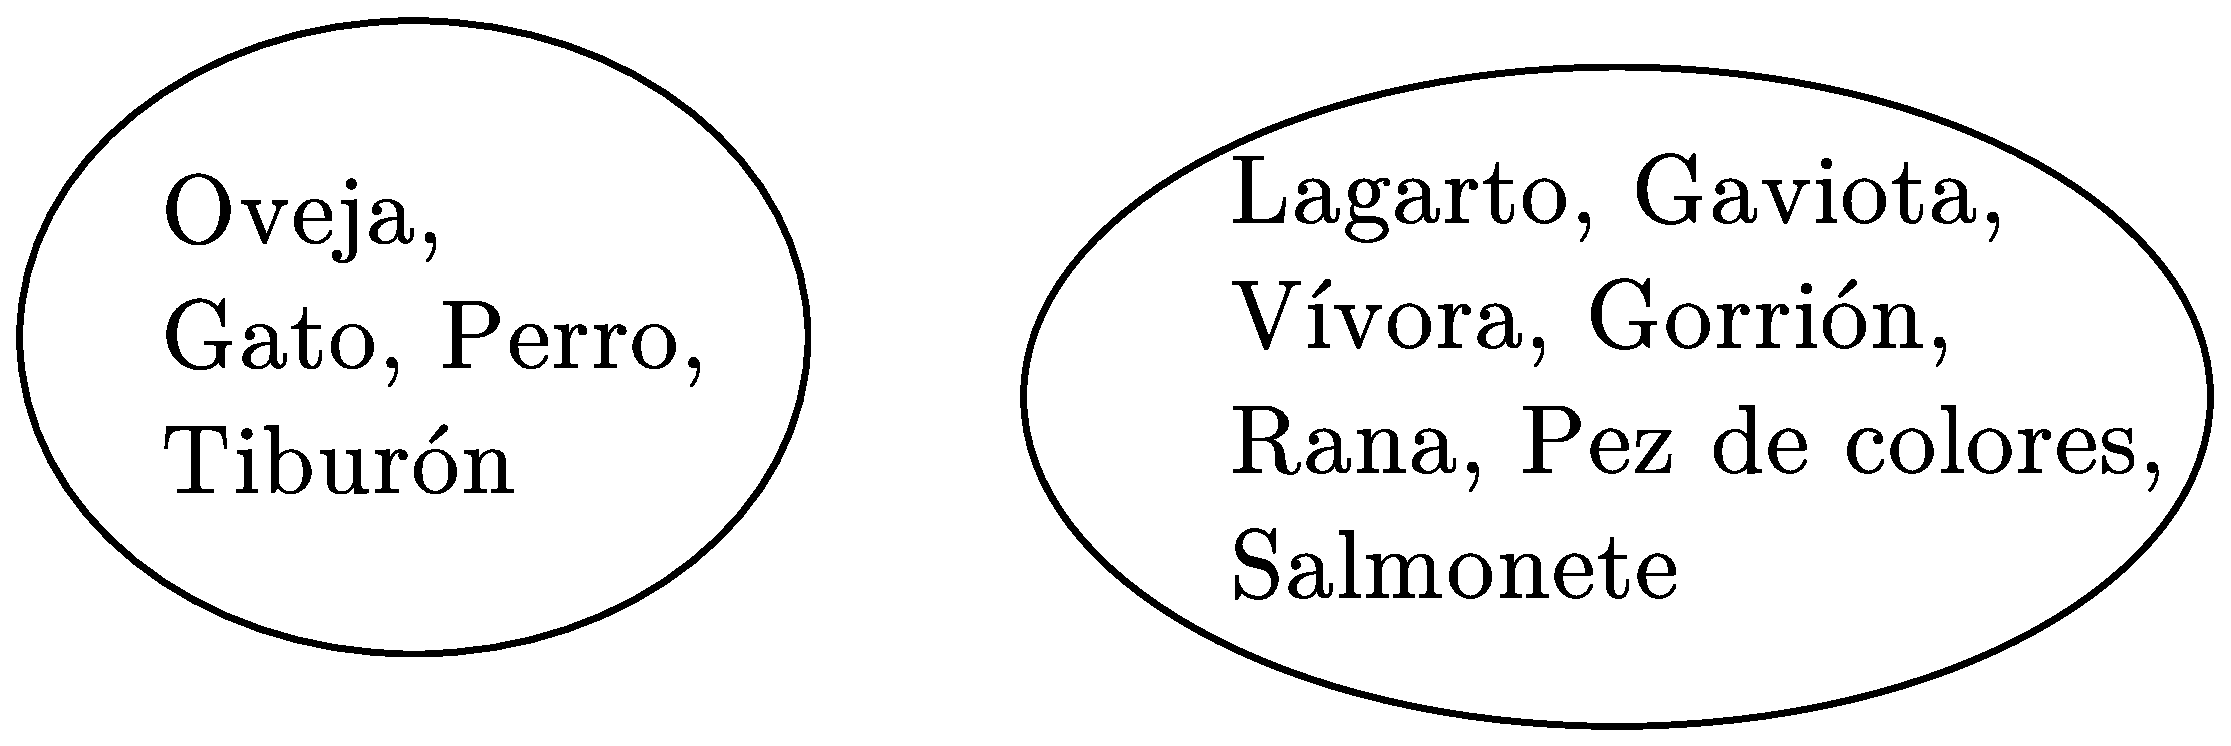
\includegraphics[scale=0.35,type=png,ext=.png,read=.png]{figures/ejemplo1}
\caption{Clustering usando como criterio la manera que llevan a cabo su descendencia}
\label{fig:ejemplo1}
\end{figure}

\begin{figure}[htb]
\centering
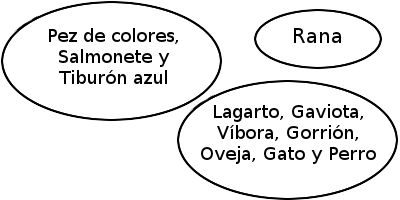
\includegraphics[scale=0.35,type=png,ext=.png,read=.png]{figures/ejemplo2}
\caption{Clustering usando como criterio la existencia de pulmones}
\label{fig:ejemplo2}
\end{figure}

\begin{figure}[htb]
\centering
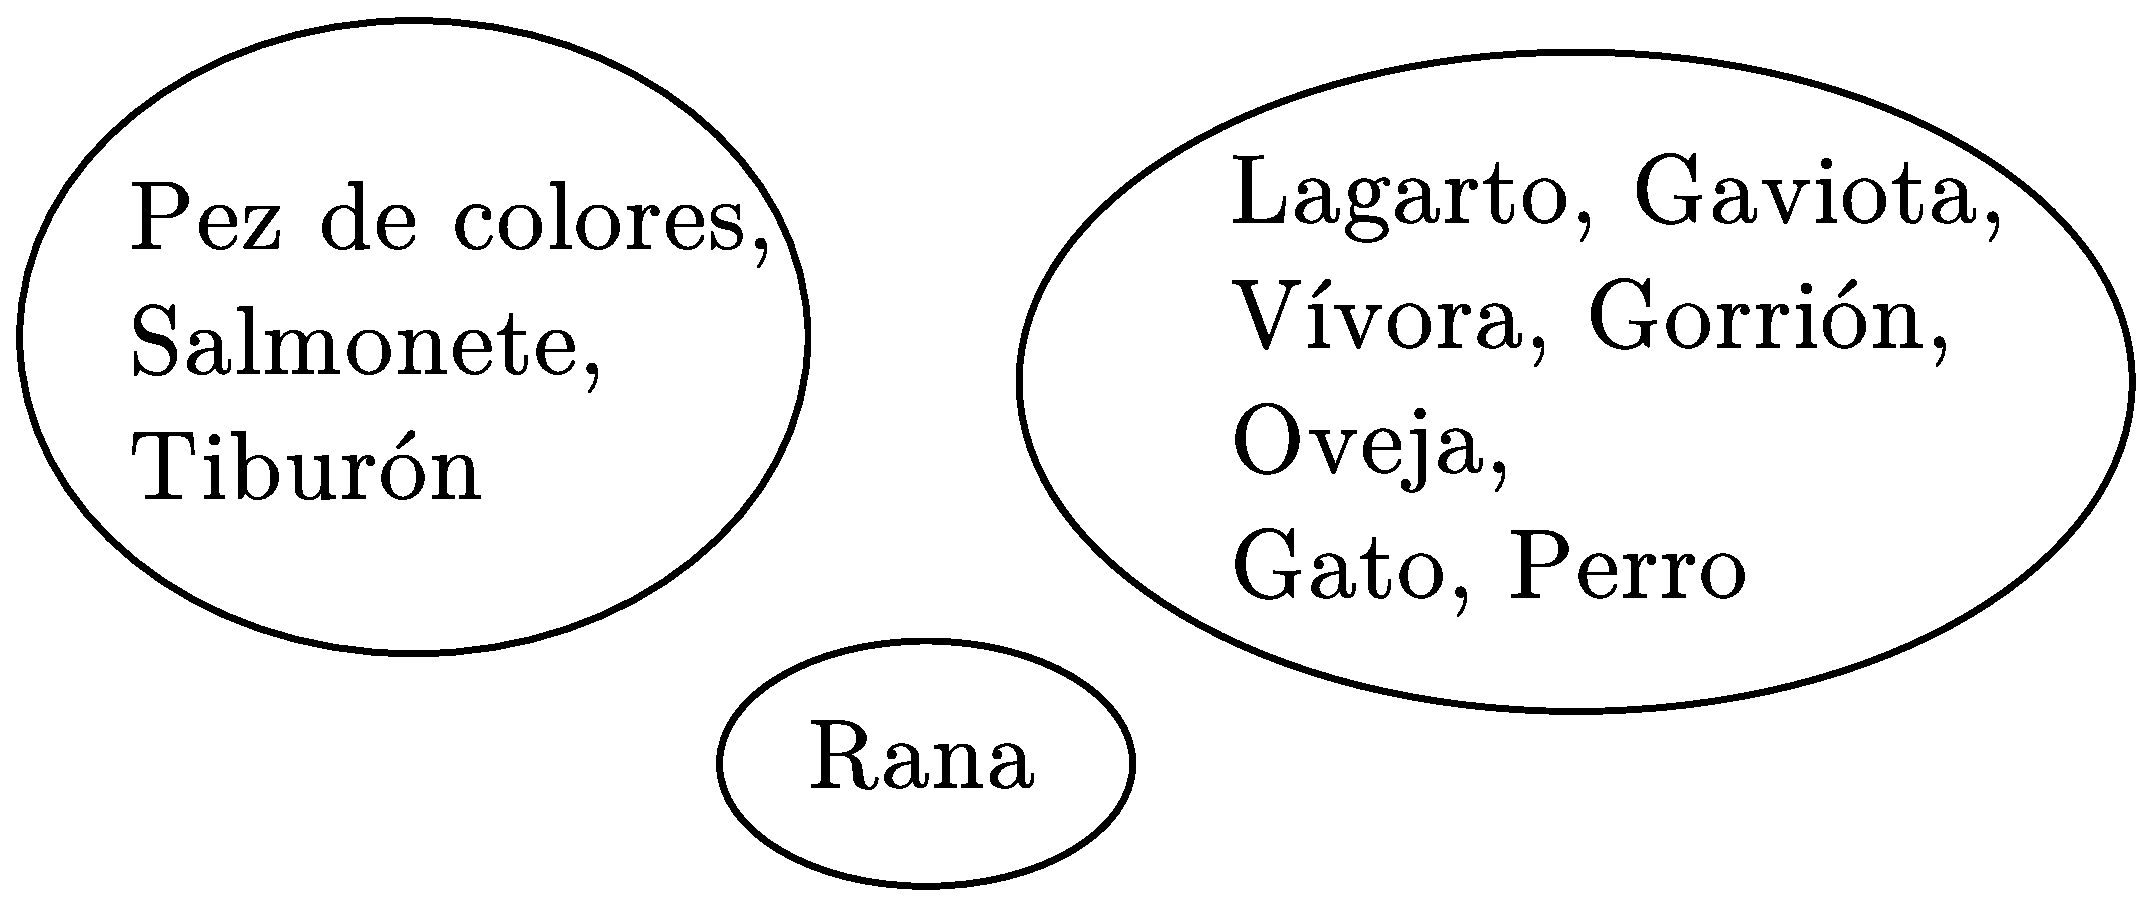
\includegraphics[scale=0.35,type=png,ext=.png,read=.png]{figures/ejemplo3}
\caption{Clustering usado como criterio el ambiente donde viven}
\label{fig:ejemplo3}
\end{figure}

Se puede ver que gracias a la falta de un criterio universal para el clustering,
 \'esta es muy subjetiva en muchos casos.

\item Se puede ver desde el punto de vista de aprendizaje autom\'atico, donde los clusters
correponden a patrones escondidos en los datos, la b\'usqueda de clusters 
es una especie de aprendizaje no supervisado, y el sistema resultante representa
un concepto de datos. Es importante entender la diferencia
entre clustering (aprendizaje no supervisado) y clasificaci\'on supervisada 
(an\'alisis discriminante). En esta \'ultima, se provee una colecci\'on patrones etiquetados
(preclasificados); el problema es etiquetar a un patr\'on recien encontrado, a\'un no etiquetado. 
Tipicamente, los patrones etiquetados (entrenamiento) ya dados son usados para obtener
la descripciones de las clases, que a su vez se utilizan para etiquetar un nuevo patr\'on.
En este caso de clustering, el problema consiste en agrupar una colecci\'on de patrones no etiquetados
en clusters significativos. En este sentidos, las etiquetas se asocian con los clusters tambi\'en,
pero esta categor\'ia de etiquetas son basados en datos, es decir, que se obtienen unicamente
de \'estos.

\item Un algoritmos de clustering se espera que descubra el agrupamiento natural
(pertinente a la noci\'on de los humanos clustering) que existe en una conjunto 
de patrones o puntos de datos. Cada patr\'on puede ser identificado como un punto en un hiperespacio,
llamado espacio de caracter\'isticas, abarcado por las caracter\'isticas asociadas a \'el. La entrada
es un conjunto esos puntos en el espacio carater\'istico multidimensional. Un algoritmo ideal de 
clustering preciso debe presentar como su salida, la etiqueda para cada patr\'on, es decir,
el cluster a cual pertenece cada punto.

\end{itemize}

\'Este problema a sido abordado por diversos campos del conocimiento como la estad\'istica
(an\'aslisis multivariado), teor\'ia de grafos, computaci\'on evolutiva, redes neurales y
as\'i sucesivamente\cite{SwAjAm2009}. Entre sus aplicaciones se encuentra la miner\'ia de datos, expresi\'on de los genes, 
segmentaciones de clientes y procesamiento de im\'agenes, muchas otras. \cite{GaChJi2007}

En especial llama la atenci\'on el \'ultimo mencionado. El procesamiento de im\'agenes es fundamental para los
humanos. Su importancia radica en que la salida puede ser usada como la entrada para 
un modelo basado en sistemas de reconocimiento de objetos.
\'Esto le da una gama de aplicaciones gigantescas: cualquier tipo de reconicimiento de im\'agenes.
Tambi\'en en el \'area m\'edica puede ayudar a encontrar regiones en las im\'agenes que sean tumores,
que posiblemente humano no logre identificar, lo que es extremadamente
\'util.

Brucker en \cite{Br1978} ilustr\'o que el problema es NP-hard cuando el n\'umero 
de clusters excede 3.

\subsection{Definici\'on} \label{sect:dclustdef}

Siguiendo con \cite{SwAjAm2009} antes de dar un definici\'on matem\'atica al problema hay que hablar de 
los siguientes t\'erminos que van a ser usados a trav\'es de la tesis:

\begin{itemize}

\item {\bf Patr\'on o vector caracter\'istico:} Se va a encargar de abstraer matem\'aticamente las
caracter\'isticas que poseen los objetos a los cuales se les har\'a el clustering.

\item {\bf Caracter\'istica:} Es una componente de un patr\'on. \'Esta representa
la base usada para clasificaci\'on de los patrones.

\item {\bf Cluster:} Es un grupo de patrones similares, y los patrones de dos clusters 
distintos no deben ser similares.

\item {\bf Hard clustering:} Cada patr\'on se asigna solamente a un cluster.

\item {\bf Medici\'on de distancia:} Es la m\'etrica con la cual se va a evaluar
la disimilaridad entre los patrones. M\'as adelante se habl\'a en m\'as detalle.

\end{itemize}

Ahora se puede dar una definici\'on formal al problema:

Sea $P = \{ P_1, P_2, \dots , P_N\}$ un conjunto de N patrones, 
donde cada uno tiene M caracter\'isticas. Éstos pueden
ser reprentados por una matriz Z$_{NxM}$. El vector de la fila i caracteriza al 
patr\'on i del conjunto P y cada elemento Z$_{i,j}$ en Z$_i$ su caracter\'istica j.
Dada tal matriz Z$_{NxM}$ la idea es que un algoritmo de clustering intente hallar
el particionamiento $C = \{ C_1, C_2, \dots , C_K \}$ tal que los patrones
en el mismo cluster C$_i$ su similaridad sea la mayor y entre clusteres diferentes
sean lo más disimilar:

\begin{enumerate}

\item Cada cluster debe tener por lo menos un patr\'on asignado:

$\forall i | i \in \{1, 2, \dots, K\} : C_i \neq \emptyset$

\item Dos patrones distintos no tienen ning\'un patr\'on en com\'un:

$\forall i,j | i,j\in \{1, 2, \dots, K\} \land i \neq j:  C_i \cap C_j \neq \emptyset$

\item Cada patr\'on debe estar asignado a un cluster:

$\bigcup_{i=1}^{K} C_i = P$

\end{enumerate}

Dado que el conjunto de datos dados puede ser partidionado de varias maneras
manteniendo las propiedades de arriba, es necesaria una función objetico o en otras palabras
una medida de que tan buena es la partici\'on. El problema se comvierte en hallar
una partici\'on C$^*$  \'optima o lo m\'as cercano a ella en comparaci\'on a 
las otras soluciones posible $C = \{ C^1, C^2, \dots, C^{T(N,K)} \}$ donde 
$T(N,K) = { {1 \over K!} \times {\sum_{i=1}^{K} (-1)^i  \binom{K}{i} (K-i)^i} }$
es el n\'umero de particiones posibles. \'Esto es lo mismo que optimizar $f(Z_{NxM}, PC)$,
donde PC es un partici\'on del conjunto C y $f$ es una funci\'on objetivo que
cuantifica la calidad del particionamiento en base a la similaridad o disimilaridad
de los patrones.
